% GNUPLOT: LaTeX picture with Postscript
\begingroup
  \makeatletter
  \providecommand\color[2][]{%
    \GenericError{(gnuplot) \space\space\space\@spaces}{%
      Package color not loaded in conjunction with
      terminal option `colourtext'%
    }{See the gnuplot documentation for explanation.%
    }{Either use 'blacktext' in gnuplot or load the package
      color.sty in LaTeX.}%
    \renewcommand\color[2][]{}%
  }%
  \providecommand\includegraphics[2][]{%
    \GenericError{(gnuplot) \space\space\space\@spaces}{%
      Package graphicx or graphics not loaded%
    }{See the gnuplot documentation for explanation.%
    }{The gnuplot epslatex terminal needs graphicx.sty or graphics.sty.}%
    \renewcommand\includegraphics[2][]{}%
  }%
  \providecommand\rotatebox[2]{#2}%
  \@ifundefined{ifGPcolor}{%
    \newif\ifGPcolor
    \GPcolortrue
  }{}%
  \@ifundefined{ifGPblacktext}{%
    \newif\ifGPblacktext
    \GPblacktexttrue
  }{}%
  % define a \g@addto@macro without @ in the name:
  \let\gplgaddtomacro\g@addto@macro
  % define empty templates for all commands taking text:
  \gdef\gplbacktext{}%
  \gdef\gplfronttext{}%
  \makeatother
  \ifGPblacktext
    % no textcolor at all
    \def\colorrgb#1{}%
    \def\colorgray#1{}%
  \else
    % gray or color?
    \ifGPcolor
      \def\colorrgb#1{\color[rgb]{#1}}%
      \def\colorgray#1{\color[gray]{#1}}%
      \expandafter\def\csname LTw\endcsname{\color{white}}%
      \expandafter\def\csname LTb\endcsname{\color{black}}%
      \expandafter\def\csname LTa\endcsname{\color{black}}%
      \expandafter\def\csname LT0\endcsname{\color[rgb]{1,0,0}}%
      \expandafter\def\csname LT1\endcsname{\color[rgb]{0,1,0}}%
      \expandafter\def\csname LT2\endcsname{\color[rgb]{0,0,1}}%
      \expandafter\def\csname LT3\endcsname{\color[rgb]{1,0,1}}%
      \expandafter\def\csname LT4\endcsname{\color[rgb]{0,1,1}}%
      \expandafter\def\csname LT5\endcsname{\color[rgb]{1,1,0}}%
      \expandafter\def\csname LT6\endcsname{\color[rgb]{0,0,0}}%
      \expandafter\def\csname LT7\endcsname{\color[rgb]{1,0.3,0}}%
      \expandafter\def\csname LT8\endcsname{\color[rgb]{0.5,0.5,0.5}}%
    \else
      % gray
      \def\colorrgb#1{\color{black}}%
      \def\colorgray#1{\color[gray]{#1}}%
      \expandafter\def\csname LTw\endcsname{\color{white}}%
      \expandafter\def\csname LTb\endcsname{\color{black}}%
      \expandafter\def\csname LTa\endcsname{\color{black}}%
      \expandafter\def\csname LT0\endcsname{\color{black}}%
      \expandafter\def\csname LT1\endcsname{\color{black}}%
      \expandafter\def\csname LT2\endcsname{\color{black}}%
      \expandafter\def\csname LT3\endcsname{\color{black}}%
      \expandafter\def\csname LT4\endcsname{\color{black}}%
      \expandafter\def\csname LT5\endcsname{\color{black}}%
      \expandafter\def\csname LT6\endcsname{\color{black}}%
      \expandafter\def\csname LT7\endcsname{\color{black}}%
      \expandafter\def\csname LT8\endcsname{\color{black}}%
    \fi
  \fi
    \setlength{\unitlength}{0.0500bp}%
    \ifx\gptboxheight\undefined%
      \newlength{\gptboxheight}%
      \newlength{\gptboxwidth}%
      \newsavebox{\gptboxtext}%
    \fi%
    \setlength{\fboxrule}{0.5pt}%
    \setlength{\fboxsep}{1pt}%
    \definecolor{tbcol}{rgb}{1,1,1}%
\begin{picture}(3400.00,2266.00)%
    \gplgaddtomacro\gplbacktext{%
      \csname LTb\endcsname%%
      \put(300,384){\makebox(0,0)[r]{\strut{}$0$}}%
      \put(300,574){\makebox(0,0)[r]{\strut{}$1$}}%
      \put(300,764){\makebox(0,0)[r]{\strut{}$2$}}%
      \put(300,954){\makebox(0,0)[r]{\strut{}$3$}}%
      \put(300,1145){\makebox(0,0)[r]{\strut{}$4$}}%
      \put(300,1335){\makebox(0,0)[r]{\strut{}$5$}}%
      \put(300,1525){\makebox(0,0)[r]{\strut{}$6$}}%
      \put(300,1715){\makebox(0,0)[r]{\strut{}$7$}}%
      \put(300,1905){\makebox(0,0)[r]{\strut{}$8$}}%
      \put(372,264){\makebox(0,0){\strut{}$0$}}%
      \put(672,264){\makebox(0,0){\strut{}$2$}}%
      \put(973,264){\makebox(0,0){\strut{}$4$}}%
      \put(1273,264){\makebox(0,0){\strut{}$6$}}%
      \put(1574,264){\makebox(0,0){\strut{}$8$}}%
      \put(1874,264){\makebox(0,0){\strut{}$10$}}%
      \put(2174,264){\makebox(0,0){\strut{}$12$}}%
      \put(2475,264){\makebox(0,0){\strut{}$14$}}%
      \put(2775,264){\makebox(0,0){\strut{}$16$}}%
      \put(2847,384){\makebox(0,0)[l]{\strut{}$0$}}%
      \put(2847,574){\makebox(0,0)[l]{\strut{}$8$}}%
      \put(2847,764){\makebox(0,0)[l]{\strut{}$16$}}%
      \put(2847,954){\makebox(0,0)[l]{\strut{}$24$}}%
      \put(2847,1145){\makebox(0,0)[l]{\strut{}$32$}}%
      \put(2847,1335){\makebox(0,0)[l]{\strut{}$40$}}%
      \put(2847,1525){\makebox(0,0)[l]{\strut{}$48$}}%
      \put(2847,1715){\makebox(0,0)[l]{\strut{}$56$}}%
      \put(2847,1905){\makebox(0,0)[l]{\strut{}$64$}}%
    }%
    \gplgaddtomacro\gplfronttext{%
      \csname LTb\endcsname%%
      \put(2208,1782){\makebox(0,0)[r]{\strut{}latency}}%
      \csname LTb\endcsname%%
      \put(2208,1662){\makebox(0,0)[r]{\strut{}throughput}}%
      \csname LTb\endcsname%%
      \put(114,1144){\rotatebox{-270.00}{\makebox(0,0){\strut{}cycles/iter}}}%
      \put(3123,1144){\rotatebox{-270.00}{\makebox(0,0){\strut{}flops/cycle}}}%
      \put(1573,84){\makebox(0,0){\strut{}variables}}%
      \put(1573,2085){\makebox(0,0){\strut{}a compile-time constant number of variables}}%
    }%
    \gplbacktext
    \put(0,0){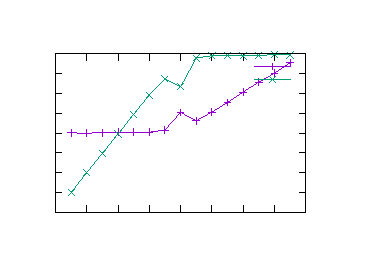
\includegraphics[width={170.00bp},height={113.30bp}]{out/tex/data/06axpb//cpu_latency_throughput_simd_c_big}}%
    \gplfronttext
  \end{picture}%
\endgroup
